\documentclass[journal,12pt,twocolumn]{IEEEtran}
\usepackage{romannum}
\usepackage{float}
\usepackage{setspace}
\usepackage{gensymb}
\singlespacing
\usepackage[cmex10]{amsmath}
\usepackage{amsthm}
\usepackage{mathrsfs}
\usepackage{txfonts}
\usepackage{stfloats}
\usepackage{bm}
\usepackage{cite}
\usepackage{cases}
\usepackage{subfig}
\usepackage{longtable}
\usepackage{multirow}
\usepackage{enumitem}
\usepackage{mathtools}
\usepackage{steinmetz}
\usepackage{tikz}
\usepackage{circuitikz}
\usepackage{verbatim}
\usepackage{tfrupee}
\usepackage[breaklinks=true]{hyperref}
\usepackage{tkz-euclide}
\usetikzlibrary{calc,math}
\usepackage{listings}
    \usepackage{color}                                            %%
    \usepackage{array}                                            %%
    \usepackage{longtable}                                        %%
    \usepackage{calc}                                             %%
    \usepackage{multirow}                                         %%
    \usepackage{hhline}                                           %%
    \usepackage{ifthen}                                           %%
  %optionally (for landscape tables embedded in another document): %%
    \usepackage{lscape}     
\usepackage{multicol}
\usepackage{chngcntr}
\DeclareMathOperator*{\Res}{Res}
\renewcommand\thesection{\arabic{section}}
\renewcommand\thesubsection{\thesection.\arabic{subsection}}
\renewcommand\thesubsubsection{\thesubsection.\arabic{subsubsection}}

\renewcommand\thesectiondis{\arabic{section}}
\renewcommand\thesubsectiondis{\thesectiondis.\arabic{subsection}}
\renewcommand\thesubsubsectiondis{\thesubsectiondis.\arabic{subsubsection}}

% correct bad hyphenation here
\hyphenation{op-tical net-works semi-conduc-tor}
\def\inputGnumericTable{}                                 %%

\lstset{
frame=single, 
breaklines=true,
columns=fullflexible
}

\begin{document}


\newtheorem{theorem}{Theorem}[section]
\newtheorem{problem}{Problem}
\newtheorem{proposition}{Proposition}[section]
\newtheorem{lemma}{Lemma}[section]
\newtheorem{corollary}[theorem]{Corollary}
\newtheorem{example}{Example}[section]
\newtheorem{definition}[problem]{Definition}
\newcommand{\BEQA}{\begin{eqnarray}}
\newcommand{\EEQA}{\end{eqnarray}}
\newcommand{\define}{\stackrel{\triangle}{=}}

\bibliographystyle{IEEEtran}
\providecommand{\mbf}{\mathbf}
\providecommand{\pr}[1]{\ensuremath{\Pr\left(#1\right)}}
\providecommand{\qfunc}[1]{\ensuremath{Q\left(#1\right)}}
\providecommand{\sbrak}[1]{\ensuremath{{}\left[#1\right]}}
\providecommand{\lsbrak}[1]{\ensuremath{{}\left[#1\right.}}
\providecommand{\rsbrak}[1]{\ensuremath{{}\left.#1\right]}}
\providecommand{\brak}[1]{\ensuremath{\left(#1\right)}}
\providecommand{\lbrak}[1]{\ensuremath{\left(#1\right.}}
\providecommand{\rbrak}[1]{\ensuremath{\left.#1\right)}}
\providecommand{\cbrak}[1]{\ensuremath{\left\{#1\right\}}}
\providecommand{\lcbrak}[1]{\ensuremath{\left\{#1\right.}}
\providecommand{\rcbrak}[1]{\ensuremath{\left.#1\right\}}}
\theoremstyle{remark}
\newtheorem{rem}{Remark}
\newcommand{\sgn}{\mathop{\mathrm{sgn}}}
\providecommand{\abs}[1]{\left\vert#1\right\vert}
\providecommand{\res}[1]{\Res\displaylimits_{#1}} 
\providecommand{\norm}[1]{\left\lVert#1\right\rVert}
\providecommand{\mtx}[1]{\mathbf{#1}}
\providecommand{\mean}[1]{E\left[ #1 \right]}
\providecommand{\fourier}{\overset{\mathcal{F}}{ \rightleftharpoons}}
\providecommand{\system}{\overset{\mathcal{H}}{ \longleftrightarrow}}
\newcommand{\solution}{\noindent \textbf{Solution: }}
\newcommand{\cosec}{\,\text{cosec}\,}
\providecommand{\dec}[2]{\ensuremath{\overset{#1}{\underset{#2}{\gtrless}}}}
\newcommand{\myvec}[1]{\ensuremath{\begin{pmatrix}#1\end{pmatrix}}}
\newcommand{\mydet}[1]{\ensuremath{\begin{vmatrix}#1\end{vmatrix}}}
\numberwithin{equation}{subsection}
\makeatletter
\@addtoreset{figure}{problem}
\makeatother

\let\StandardTheFigure\thefigure
\let\vec\mathbf
\renewcommand{\thefigure}{\theproblem}



\def\putbox#1#2#3{\makebox[0in][l]{\makebox[#1][l]{}\raisebox{\baselineskip}[0in][0in]{\raisebox{#2}[0in][0in]{#3}}}}
     \def\rightbox#1{\makebox[0in][r]{#1}}
     \def\centbox#1{\makebox[0in]{#1}}
     \def\topbox#1{\raisebox{-\baselineskip}[0in][0in]{#1}}
     \def\midbox#1{\raisebox{-0.5\baselineskip}[0in][0in]{#1}}

\vspace{3cm}


\title{Assignment 1}
\author{Jaswanth Chowdary Madala}





% make the title area
\maketitle

\newpage

%\tableofcontents

\bigskip

\renewcommand{\thefigure}{\theenumi}
\renewcommand{\thetable}{\theenumi}

\begin{enumerate}
\item In the following figure for the triangle ABC, which of the following is not true:

(A) $\overrightarrow{AB}+\overrightarrow{BC}+\overrightarrow{CA} = \overrightarrow{0}$

(B) $\overrightarrow{AB}+\overrightarrow{BC}-\overrightarrow{AC} = \overrightarrow{0}$

(C) $\overrightarrow{AB}+\overrightarrow{BC}+\overrightarrow{AC} = \overrightarrow{0}$

(D) $\overrightarrow{AB}-\overrightarrow{CB}+\overrightarrow{CA} = \overrightarrow{0}$

\begin{figure}[h]
\centering
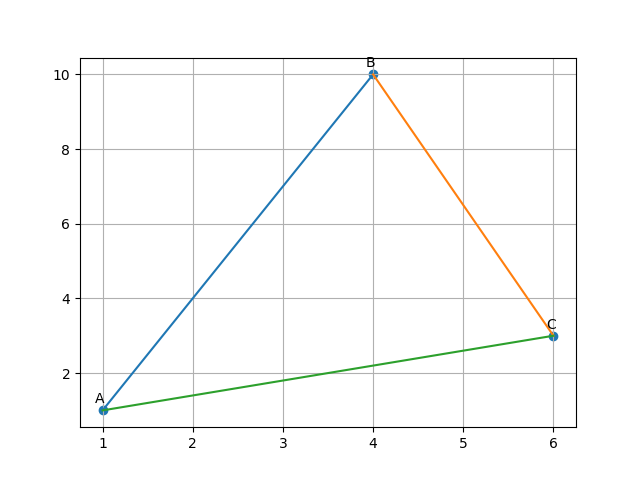
\includegraphics[width = \columnwidth]{./figs/triangle.png}
\caption{}
\end{figure}
\textbf{Solution:} We know that,
\begin{align}
\overrightarrow{AB} = \vec{B} - \vec{A}\\
\overrightarrow{BC} = \vec{C} - \vec{B}\\
\overrightarrow{CA} = \vec{A} - \vec{C}
\end{align}
By usinig this we verify each of the given option

\begin{enumerate}
\item 
\begin{align}
\overrightarrow{AB}+\overrightarrow{BC}+\overrightarrow{CA} &=
\vec{B}-\vec{A} + \vec{C} - \vec{B} + \vec{A} - \vec{C}\\
 &= 0
\end{align}
Option A is correct.

\item
\begin{align}
\overrightarrow{AB}+\overrightarrow{BC}-\overrightarrow{AC} &=
\vec{B}-\vec{A} + \vec{C} - \vec{B} - (\vec{C} - \vec{A})\\
 &= 0
\end{align}
Option B is correct.

\item 
\begin{align}
\overrightarrow{AB}+\overrightarrow{BC}+\overrightarrow{AC} &=
\vec{B}-\vec{A} + \vec{C} - \vec{B} + \vec{C} - \vec{A}\\
 &= 2(\vec{C}-\vec{A})
\end{align}
Option C is incorrect.

\item
\begin{align}
\overrightarrow{AB}-\overrightarrow{CB}+\overrightarrow{CA} &=
\vec{B}-\vec{A} - (\vec{B} - \vec{C}) + \vec{A} - \vec{C}\\
 &= 0
\end{align}
\end{enumerate}
Option D is correct.

The options A, B, D are correct and the option C is incorrect.\\

Verification: Let us take an example to verify 
\begin{align}
\vec{A} = \myvec{1\\1} \\
\vec{B} = \myvec{3\\1} \\
\vec{c} = \myvec{6\\6} \\
\overrightarrow{AB} = \vec{B} - \vec{A} = \myvec{2\\0} \\
\overrightarrow{BC} = \vec{C} - \vec{B} = \myvec{3\\5} \\
\overrightarrow{CA} = \vec{A} - \vec{C} = \myvec{-5\\-5} 
\end{align}

\begin{align}
\overrightarrow{AB}+\overrightarrow{BC}+\overrightarrow{CA} = \myvec{2+3+(-5) \\ 0+5+(-5)} = \myvec{0 \\0}
\end{align}
Similarly other options can be verified.

\end{enumerate}
\end{document}